% !TEX root =../LibroTipoETSI.tex
\chapter{PF\_RING}\LABCHAP{PFRING}
\pagestyle{esitscCD}

\epigraph{In almost every computation a great variety of arrangements for the succession of the processes is possible, 
and various considerations must influence the selections amongst them for the purposes of a calculating engine. One 
essential object is to choose that arrangement which shall tend to reduce to a minimum the time necessary for completing 
the calculation.}{Ada Lovelace}

%\lettrine[lraise=0.7, lines=1, loversize=-0.25]{E}{l} 
\lettrine[lraise=-0.1, lines=2, loversize=0.25]{E}n un sistema de monitorización de tráfico, la captura de paquetes es 
un proceso vital. Si se quiere capturar tráfico a una velocidad aceptable, superiores a 1Gbps, es necesario que todo el 
proceso de captura de paquetes esté bien diseñado y sea eficiente. De no serlo, enseguida comenzaremos a notar 
pérdidas de paquetes, y nuestra monitorización no será efectiva.

%TODO unir con lo demás
Ya hemos cubierto la eficiencia en términos de procesamiento de paquetes en los anteriores capítulos. 

\gls{PFRING} es, según su autor Luca Deri, una tecnología que persigue capturar tráfico a $10G$ sin necesitar 
tarjetas especializadas, sin pérdidas y bajo cualquier circunstancia del tráfico, de forma que sea posible crear sondas 
de tráfico software con el mismo rendimiento que las basadas en hardware \cite{LucaDeriPFRING}.

A lo largo de este capítulo, %TODO

\section{Conceptos preliminares}\SEC{PFRINGConceptosPreliminares}
Antes de explicar cómo consigue \texttt{PF\_RING} mejorar la velocidad de captura de paquetes, es necesario explicar 
algunos conceptos y procedimientos relativos a ella. Hacerlo en esta sección previa ayudará a abstraernos de ellas a 
la hora de explicar dichas mejoras.

\subsection{Núcleo del SO Linux y su diseño modular}\index{Núcleo del Sistema Operativo}
El núcleo del sistema operativo es el encargado de abstraer las relaciones con el hardware, el planificador de tareas, 
y demás componentes que se crean necesarios a la hora de diseñarlo, de las aplicaciones del espacio de usuario.

Por ejemplo, para enviar un dato a la red, es posible que la operación necesaria sea colocar un byte determinado en una 
posición de memoria. Sin embargo, para otra tarjeta mas antigua, se debe colocar un byte distinto. El núcleo abstraerá 
estas dos formas de comunicarse con la tarjeta, y presentará a los programas de usuario un método homogéneo 
\texttt{envía}.

Por otro lado, el núcleo es también responsable de gestionar, como componente hardware que es, la memoria disponible. 
Si algún proceso requiere memoria, es necesario que se la pida al núcleo, que se encargará de asignar la memoria de 
procesos de una forma ordenada y coherente.

Además, Linux es también responsable de gestionar el planificador de tareas. Éste es el que decide qué aplicación se 
ejecutará en qué momento, y cuánto tiempo de ejecución le corresponde hasta tener que dejar paso a otra. 

\subsubsection{Módulos del kernel}\index{Módulos de Linux}
Linux es un \gls{SO} modular. Esto quiere decir que parte de sus procedimientos pueden ser exportados a un módulo, ser 
cargado de forma dinámica, y ser descargado cuando ya no sea requerido, lo cual permite ahorrar recursos.

Por ejemplo, un controlador es código que se ejecuta a nivel de núcleo y sirve para lograr manejar un dispositivo desde 
una interfaz común. Los controladores suelen venir en forma de módulos. De otra forma, sería necesario compilar un 
núcleo distinto por cada configuración hardware distinta, o bien cargar todos los módulos aunque no se usen, lo cual 
sería un desperdicio de recursos.

\subsection{Interrupción}\index{Interrupciones}
Desde un punto de vista de ``caja negra'', una interrupción funciona de la misma manera que las señales explicadas en 
\SSEC{SIGALRM}, pero a nivel del núcleo del \gls{SO}. Cada interrupción tiene asociada un número que identifica a una 
función. En el momento que el núcleo recibe una interrupción, ejecutará la función asociada.

Normalmente, para lanzar interrupciones en el núcleo se ejecuta una instrucción concreta del procesador, que puede ser 
lanzada desde el núcleo o desde el espacio de usuario, y necesita tener en registros o en memoria los parámetros 
necesarios para saber qué hacer con ella

\subsection{Llamada al sistema}\index{Llamadas al Sistema}
Una llamada al sistema es una forma de realizar operaciones a nivel de núcleo. Por ejemplo, un sistema no puede 
asignarse para sí una porción de memoria: deberá llamar al núcleo y pedirla. Del mismo modo, no puede abrir 
directamente un fichero en el sistema de archivos, ni colocarse en una posición concreta del planificador. Ni siquiera 
puede leer directamente la hora del sistema.

Para realizar este tipo de tareas, es necesario que el programa lance una llamada al sistema. Cuando esto ocurre, una 
interrupción es lanzada al núcleo indicando que un programa necesita realizar tareas con privilegios elevados. A la 
hora de gestionarla, el núcleo decide si puede o no realizarla, y le devolverá uno o más valores.

No obstante, las llamadas al sistema pueden volverse un cuello de botella ya que, de la misma forma que lo son las 
señales, las llamadas al sistema e interrupciones son complejas y Linux las realiza con cuidado y, posiblemente, 
lentitud.

\subsection{Programador de tareas}\index{Programador de tareas}
El programador de tareas es el elemento de Linux que decide qué programa debe ejecutarse en qué intervalo de tiempo. Es 
posible modificar su comportamiento, y existen instrucciones específicas para que un programa continúe su ejecución en 
un número determinado de segundos. Es lo que se conoce como ``dormir al programa''.

A cada cambio de tarea, es necesario que el procesador \emph{cambie de contexto}\index{Cambio de contexto}. Cuando un 
programa es ejecutado, y le toca el turno a otro programa, es necesario que los registros que él tuviese, su puntero a 
pila, y, en resumen, el estado actual del programa, se almacene en una sección de memoria y de paso al siguiente 
programa en el planificador.

Así pues, es importante conocer los detalles del programador de tareas para ajustarlo: Una frecuencia de cambio elevada 
provocará muchos cambios de contexto y pérdidas de rendimiento por ello, pero una muy baja puede dedicar demasiado 
tiempo a unos programas, y demasiado poco a otros.

\subsection{Memoria mapeada o mapeo de memoria}\index{Mapeo de Memoria}
Como ya hemos dicho, sólo el núcleo puede acceder a toda la memoria sin restricciones. Para que una aplicación acceda a 
una región de memoria cualquiera, es necesario que ésta sea otorgada a la misma por el núcleo. Es más, cada acceso a 
la memoria es, en última instancia, monitorizada por el núcleo, de forma que no se produzcan accesos a zonas de memoria 
no autorizadas.

Esto conlleva un problema. Si una aplicación necesita acceder a memoria que hasta ahora poseía el núcleo, como un 
fichero cargado en memoria, es necesario copiar la región de memoria desde el espacio del núcleo hasta la memoria del 
espacio de usuario.

La técnica de \gls{mmap}\index{Memory Mapping} consiste en asignar una región de memoria que actúe de acceso directo a 
cualquier cosa. Por ejemplo, podríamos mapear un fichero en memoria, de forma que escribir en la posición $0xF000$ de 
memoria sea escribir en el primer byte del fichero, $0xF0001$ en el segundo, y así sucesivamente. De esa forma, no es 
necesario copiar el fichero desde el espacio del núcleo al usuario y viceversa, sino que el mapeado de memoria se 
encarga de resolver dichas escrituras y lecturas.

\subsection{Acceso directo a memoria}
A lo largo de la operación normal de un dispositivo, éste suele necesitar copiar regiones de memoria entre la memoria 
del dispositivo y la memoria principal del sistema.

Normalmente, los procesadores tienen alguna instrucción para copiar un bloque de memoria de tamaño $N$ o, en el peor de 
los casos, de copiar la memoria a sus registros y, tras ello, volver a volcar a la memoria. Así pues, copiar una región 
de longitud $M=k\cdot N$ se reduce a ejecutar $k$ veces el comando de copia de memoria, lo cual mantiene ocupada la CPU.

\gls{DMA} es una tecnología que permite al propio dispositivo copiar su memoria a la memoria principal. De esa forma, 
el procesador sólo necesita iniciar la copia, y recibirá una notificación cuando ésta acabe (normalmente, una 
interrupción), quedando libre para realizar otras tareas.


\section{Proceso de paquetes por el núcleo linux}\LABSEC{sec:ProcesoPaquetesLinux}
El paso de paquetes a través del núcleo Linux puede ser un importante cuello de botella. Para entender cómo evitarlo, 
es necesario conocer cómo trabaja Linux con los paquetes que recibe, qué camino siguen y qué parte del mismo es el más 
costoso.

A lo largo de esta sección vemos cómo transmite Linux los paquetes desde el cable hasta la aplicación del usuario, 
usando técnicas vistas en la \SEC{PFRINGConceptosPreliminares}. Analizaremos por qué medios realiza la tarjeta de red 
la reserva de memoria, cómo se consigue una 

\subsection{Reserva de memoria para almacenar el paquete}
El primer paso en la recepción de paquetes es que éste llegue a la tarjeta de red a través de la interfaz física. Tan 
pronto como esto ocurre, y la memoria interna de la \gls{NIC} contiene el paquete completo, ésta es responsable de 
de crear una estructura de datos para almacenar el paquete en la memoria principal del sistema, y copiarlo ahí.

Esta reserva ya incluye un corte en términos de tiempo, ya que dos procesos no pueden reservar memoria al mismo tiempo. 
El sistema tiene una tabla de memoria en la que están anotados los distintos bloques que cada proceso (incluído el 
núcleo) tiene reservada. Si dos procesos reservasen al mismo tiempo, podría ocurrir que reservasen segmentos de memoria 
solapados.

Por tanto, la reserva debe ser sincronizada, y esta sincronización consume un tiempo importante. Tras ello, la copia es 
en modo \gls{DMA}, por lo que la tarjeta obtiene acceso exclusivo a esa memoria y no es necesario la intervención de la 
CPU para copiar los datos.

El paquete es entonces copiado en una estructura de datos \texttt{sk\_buff}. Dicha estructura es bastante grande, y 
puede ir creciendo a medida que lo necesita. Esto incrementa la fragmentación de memoria, ya que al crecer es posible 
que no quepa en su segmento de memoria, y deba moverse a otro segmento mayor.

Por último, existen bastantes datos de la estructura que son privados, y no deben viajar de una capa a otra en el paso 
de información. Por tanto, hay que clonar la estructura al transmitir información\footnote{Si bien hay partes de la 
misma que pueden mantenerse}, lo que redunda en más reservas y más retrasos por sincronía
\cite{skBuffLinuxFoundation}.

\subsection{Notificación del nuevo paquete}
Cuando el paquete al completo es copiado en la memoria principal, es necesario un mecanismo de notificación al 
\gls{controlador}\index{Controlador de Dispositivo} de red de Linux para que éste pueda procesarlo. Se usa, entonces, 
una interrupción hardware.

La interrupción provoca que el núcleo deje de realizar las tareas que esté haciendo para hacer caso a la llegada del 
paquete. Sin embargo, si tenemos demasiados paquetes por segundo, no dejamos a Linux avanzar, y destrozamos la 
planificación de tareas. Este hecho es conocido como Tormenta de Interrupciones\index{Tormenta de Interrupciones} o 
\emph{interrupt storm} \cite{p206}.

Una interrupción debe ser rápida, esto es, en una interrupción no podemos realizar tareas que no sean estrictamente 
necesarias, por las mismas razones que las señales en espacio de usuario. Por ello, la interrupción provoca que se 
planee una tarea con el fin de recoger el paquete, usando la función \texttt{netif\_rx}. 

A partir de ese momento, sólo cuando el planeador decida que el sistema está libre, se recogerá el paquete usando 
\texttt{packet\_rcv}, y se pasará a la pila de red de Linux.

\subsubsection{NAPI}
Para evitar la tormenta de interrupciones, se pueden utilizar técnicas como la llamada \emph{device polling}. El 
funcionamiento es el siguiente \cite{beyondDevicePolling}.
\begin{itemize}
 \item Cuando un nuevo paquete llega, la tarjeta genera una interrupción.
 \item El \gls{SO} la maneja de la siguiente forma:
 \begin{enumerate}
  \item Prohíbe (enmascara) futuras interrupciones del dispositivo.
  \item Programa una tarea para atender a la tarjeta en un futuro.
  \item Cuando la atiende, consume todos los paquetes que la tarjeta tenía pendiente, y levanta la prohibición de 
interrupciones.
 \end{enumerate}
\end{itemize}

La implementación de esta técnica en Linux es conocida como \gls{NAPI}.

Podemos ver en las figuras \FIG{InterrupcionesNIC} y \FIG{DevicePolling} las diferencias entre un canal saturado 
con un método y otro. Se observa como, en la primera figura, al núcleo no le da tiempo a procesar todos los paquetes 
del canal saturado, y sólo puede procesar una de cada dos. Sin embargo, en la segunda figura, Linux procesa los 
paquetes cuando puede, en tiempos aleatorios, y coge de una tacada todos los paquetes que necesita.

\begin{figure}[hbtp]
\centering
%\hfill
\subfloat[Interrupción]%
   {\LABFIG{InterrupcionesNIC}%
   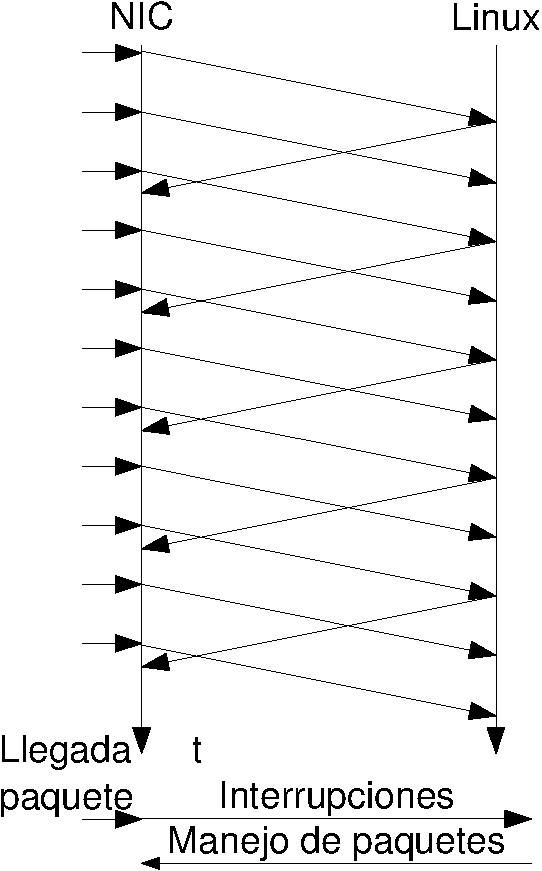
\includegraphics[width=0.30\textwidth]{CapituloPF_RING/Figuras/InterrupcionesNIC-crop}}%
\hspace{0.2\textwidth}
\subfloat[Device Polling]%
 {\LABFIG{DevicePolling}%
 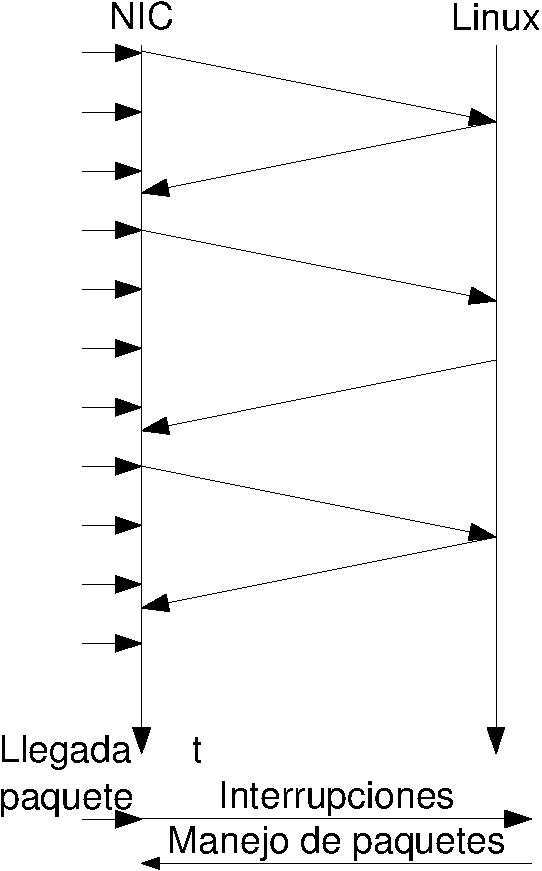
\includegraphics[width=0.30\textwidth]{CapituloPF_RING/Figuras/PollNIC-crop}}%
%
\caption{Comparativa entre los diferentes métodos de notificación de nuevos paquetes}
\end{figure}
%

Si se quiere usar NAPI, la función usada para traer paquetes es \texttt{netif\_receive\_skb}.

\subsection{Obtención del paquete por parte del kernel}
Para obtener el paquete, se añadirá a una lista doblemente enlazada, y pasará a la pila del núcleo. En la pila, el 
paquete pasará por diversos sistemas, como la parte de filtrado \emph{\gls{netfilter}}\index{Netfilter} para, 
finalmente, ser recibido por un puerto o \emph{\gls{socket}} llegar a estar listo para la recogida por parte del espacio 
de usuario \cite{p206}.

\subsection{Obtención del paquete por parte del espacio de usuario}
La recepción de paquetes en el espacio de usuario se realiza mediante la librería \emph{\gls{libpcap}}\index{libpcap}.
Para ello, \emph{\gls{libpcap}} genera un \emph{\gls{socket}} que es abstraído por un descriptor de fichero. 

La llamada al sistema \texttt{read}, y su envoltorio para \emph{sockets} \texttt{readfrom}, sirve para leer datos 
que el núcleo le pasa. Sin embargo, esta llamada es bloqueante, el hilo estará bloqueado hasta que se reciban datos por 
lo que no podremos procesar otro tipo de señales o eventos.

Por ello, existe otra llamada al sistema \texttt{select} o \texttt{poll}. Con ellas, el hilo duerme un determinado 
número de milisegundos, pero despierta si el \emph{\gls{socket}} queda listo para lectura. De esta forma, sólo 
llamaremos a \texttt{read} si es necesario, y no congelaremos el hilo.

Es importante no confundir el \texttt{poll} del espacio de usuario con el \emph{device polling}. Pese a que los 
conceptos son similares, el primero lo realiza un proceso de usuario hacia el núcleo, y el segundo lo realiza el núcleo 
hacia el dispositivo de red.

\begin{lstlisting}[language=C++,caption={Lectura desde un socket crudo}, 
breaklines=true, label=code:lecturaRawSocket,numbers=left,float=phtb]
#include<stdio.h>
#include<string.h>

#include<net/ethernet.h>
#include<sys/socket.h>
#include<arpa/inet.h>
#include<sys/ioctl.h>
#include<sys/types.h>
 
void ProcessPacket(char* , int);
 
int main(){
    size_t saddr_size, data_size;
    struct sockaddr saddr;
         
    char buffer[65536];
   
    int sock_raw = socket(AF_PACKET, SOCK_RAW, htons(ETH_P_ALL));
    setsockopt(sock_raw, SOL_SOCKET, SO_BINDTODEVICE, "eth0", 
                                               strlen("eth0")+1);
     
    if(sock_raw < 0){
        perror("Socket Error");
        return 1;
    }
    while(1){
        struct pollfd fds = { fd: sock_raw, events: POLLIN};
        const int poll_rc = poll(&fsd, 1, 1000);
        if(poll_rc == 0){
            if(poll_rc <= 0)
                perror("Poll error");
            continue;
        }
        saddr_size = sizeof(saddr);
        //Receive a packet
        data_size = recvfrom(sock_raw, buffer, 65536, 0, &saddr, 
                                       (socklen_t*)&saddr_size);
        if(data_size < 0){
            printf("Recvfrom error , failed to get packets\n");
            return 1;
        }
        //Now process the packet
        ProcessPacket(buffer , data_size);
    }
    close(sock_raw);
    return 0;
}
\end{lstlisting}

Un ejemplo de este tipo de lecturas podemos verlo en en \lstlistingname{} \ref{code:lecturaRawSocket}. En él, vemos la 
creación del socket con \texttt{socket}, la consulta de disponibilidad con \texttt{poll} y la recepción de los datos 
con \texttt{recvfrom}.

Sin embargo, este procedimiento tiene un coste oculto. A la hora de leer los datos, estos son copiados desde la 
memoria del núcleo a un buffer en espacio de usuario. Esto es, por cada paquete, estamos perdiendo tiempo y ciclos de 
CPU en copiar un dato que sólo vamos a leer.

Si, por ejemplo, queremos leer paquetes de 150kb en un enlace saturado a una velocidad de 1Gbps, estamos realizando:
\begin{itemize}
 \item $\frac{1G}{150k} \approx 7000$ llamadas al sistema con \texttt{poll} y otras tantas con \texttt{recvfrom}.
 \item Copiando entre regiones de memoria RAM a 1Gbps.
\end{itemize}

Resumiendo, por cada paquete recibido, tenemos:
\begin{enumerate}
 \item Reserva de memoria, con pérdidas por sincronización.
 \item Copia de memoria a la estructura reservada.
 \item Potencial interrupción del núcleo.
 \item Espera a la lectura del paquete, ya que ésta se programa.
 \item Llamada al sistema para conocer si el socket está listo
 \item Copia de memoria al espacio de usuario.
\end{enumerate}

\section{La alternativa: PF\_RING}\LABSEC{La alternativa: PF RING}
Luca Deri propuso crear un camino directo desde la tarjeta de red hasta el espacio de usuario, que evitase realizar 
todas las operaciones ineficientes que Linux necesita.

Para ello, diseñó un nuevo tipo de socket: \texttt{PF\_RING}. Este viene en formato módulo, y realiza algunas 
modificaciones sobre el comportamiento normal del sistema de recogida de paquetes, con el fin de ahorrar las 
operaciones costosas y hacer más rápido el proceso de captura pasiva.

\subsection{Buffer circular}
El sistema \texttt{PF\_RING} es, en su base \cite{beyondDevicePolling}:

\begin{itemize}
  \item Se crea un nuevo tipo de socket \texttt{PF\_RING}, orientado a la captura pasiva de paquetes. Se basará 
en un buffer circular, donde los paquetes se copian a medida que llegan al sistema
  \item El anillo es reservado a la creación del socket, y liberado a la finalización. Sockets diferentes tendrán 
anillos diferentes.
  \item Los paquetes no serán enviados a la pila del núcleo por defecto, de manera que este nuevo socket no sea una 
sobrecarga sino un camino alternativo.
  \item Los paquetes serán accesibles desde el espacio de usuario vía mapeado de memoria o \texttt{mmap}\index{mmap}, 
eliminando así la copia de memoria entre el espacio del núcleo y el espacio de usuario.
  \item Se crea un hilo en el núcleo específico para obtener paquetes, por lo que no afectará tanto la programación de 
la recepción.
  \item Cuando llegan paquetes, y son copiados en el anillo, Linux desplaza hacia delante el puntero de escritura. 
Cuando son leídos del anillo, se desplaza hacia delante el puntero de lectura.
  \item Nuevos paquetes sobre-escriben paquetes antiguos. Si el anillo está lleno, los paquetes son descartados.
\end{itemize}

Como resultado, Luca Deri sigue registrando pérdidas, y observa que son debidas a la llamada \texttt{poll} de espacio 
de usuario. En ella, aunque haya paquetes esperando, se desperdician muchos ciclos de CPU. Por ello, se pregunta, antes 
de realizar la llamada, si existen paquetes en el anillo (espera activa). Si la respuesta es no, se realiza la llamada 
a \texttt{poll}.

\begin{lstlisting}[language=C++,caption={Lectura de paquetes con poll en el núcleo}, 
breaklines=true, label=code:PFRINGKernelPoll,numbers=left,float=htbp]
sockFd = socket(PF_RING, SOCK_RAW, htons(ETH_P_ALL);
   ..
ringBufferPtr = mmap(NULL, ringSize,
                     PROT_READ|PROT_WRITE,MAP_SHARED, sockFd, 0);
slotId = &ringBufferPtr->slotId;

while(1) {
    if(ringBufferPtr->slot [slotId].isFull) {
        readPacket(ringBufferPtr->slot [slotId]);
        ringBufferPtr->slot [slotId].isFull = 0;
        slotId = (slotId + 1) % ringSize;
    } else {
        /* Dormir si no hay nada */
        pfd.fd = fd;
        pfd.events = POLLIN|POLLERR;
        pfd.revents = 0;
        poll(&pfd, 1, -1);
    }
}
\end{lstlisting}

\begin{lstlisting}[language=C++,caption={Lectura de paquetes con poll en el espacio de usuario}, 
breaklines=true, label=code:PFRINGUserspacePoll,numbers=left,float=htbp]
sockFd = socket(PF_RING, SOCK_RAW, htons(ETH_P_ALL);
   ..
ringBufferPtr = mmap(NULL, ringSize,
                     PROT_READ|PROT_WRITE,MAP_SHARED, sockFd, 0);
slotId = &ringBufferPtr->slotId;

while(1) {
    if(ringBufferPtr->slot [slotId].isFull) {
        readPacket(ringBufferPtr->slot [slotId]);
        ringBufferPtr->slot [slotId].isFull = 0;
        slotId = (slotId + 1) % ringSize;
    }
}
\end{lstlisting}

Podemos ver un ejemplo de este tipo de lectura en \lstlistingname{} \ref{code:PFRINGKernelPoll}. Si trasladamos el 
polling al espacio de usuario, tendríamos que eliminar todo el bloque \texttt{else}, y quedaría como en 
\lstlistingname{} \ref{code:PFRINGUserspacePoll}.

\subsection{PF\_RING ZeroCopy}
Sin embargo, con este modelo existe aún una penalización que no hemos podido eliminar: la copia de memoria entre la 
tarjeta y el núcleo, es decir, el anillo \texttt{PF\_RING}. Si se evita esta copia, y las aplicaciones son capaces de 
acceder a la memoria de la tarjeta directamente, se evitará el uso de la CPU para esta copia, y todo el procesamiento 
se reservará a la aplicación. En el anillo sólo se almacenarán los metadatos del paquete, prácticamente, un puntero al 
mismo.

Como desventaja, en este modo de funcionamiento, sólo se permite acceder a una aplicación a la misma interfaz. Esto es, 
la interfaz sólo está disponible para operar en modo sniffer, no se podrán procesar ningún tipo de paquetes de capa de 
aplicación por el resto de aplicaciones.

Esto hace algunos años era impensable, ya que las tarjetas de red se quedarían sin capacidad rápidamente. Sin embargo, 
con el paso del tiempo la memoria se ha ido abaratando, y se ha demostrado, con el uso de esta tecnología, que recoger 
los paquetes de esta forma es perfectamente viable.

Para abrir la aplicación en modo \emph{ZeroCopy} sobre, por ejemplo, la interfaz \texttt{eth0} se ejecutará la 
aplicación con la interfaz \texttt{zc:eth0}. Por ejemplo, tcpdump es una aplicación para volcar paquetes a un fichero 
pcap o a la salida estándar. Si lo hemos compilado con soporte \texttt{PF\_RING}, y queremos abrirlo en zero copy:
\begin{quote}
 \texttt{tcpdump -i zc:eth0}
\end{quote}
Desde este momento, no podemos realizar \texttt{echo request} a la dirección ip de la interfaz, ni conectarnos por 
\texttt{\gls{ssh}}, ni nada por el estilo: tan solo esnifar tráfico por \texttt{tcpdump}. Tan pronto como la aplicación 
muera, será posible volver a acceder de forma normal a la aplicación.

Gracias a \texttt{ZeroCopy}, es posible leer paquetes en una intefaz de $10G$ a \emph{wire rate}, esto es, a la 
velocidad a la que llegan los paquetes, con cualquier tamaño de paquete \cite{PFRingZc}. A partir de esto punto, 
entonces, es posible hablar de procesar paquetes con el fin de detectar ataques \gls{DDoS}.


\subsection{PF\_RING Packet Clustering}\LABSSEC{PacketClustering}
Una aplicación que monitoriza el tráfico ve un conjunto de flujos atravesar un segmento de red. Una posible forma de 
distribuir la carga entre varios hilos sería dividir ese gran flujo en flujos pequeños, de forma que cada procesador 
ejecuta la misma aplicación, sobre distintas partes del flujo.

Es importante recordar que, en la división por flujos, si un paquete que tenga como dirección origen $IP_a$ y dirección 
destino $IP_b$ es enviado al receptor $n_0$, todos los paquetes con esa misma dirección origen y destino deberán seguir 
siendo enviados a $n_0$. Es más, como se desea registrar un flujo bidireccional, los paquetes de regreso, esto es, con 
dirección origen $IP_b$ y destino $IP_a$ también deberán volver a ser enviados a $n_0$.

Una aplicación que quisiese hacer esto debería establecer una variable cerrojo sobre un socket \texttt{PF\_RING}, e ir 
consultando paquetes. O bien, crear un hilo distribuidor, e ir separando flujos.

\begin{figure}[hbtp]
\centering
\subfloat[Sin Clustering]%
   {\begin{minipage}[t]{0.45\textwidth}
    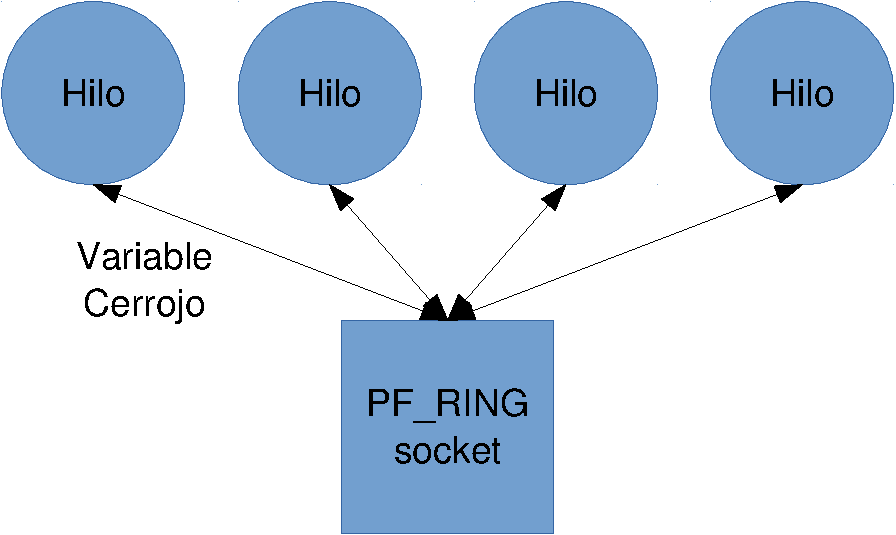
\includegraphics[width=\textwidth]{CapituloPF_RING/Figuras/CluserNoCluster-crop}%
    \LABFIG{PFRINGClusterNoCluster}
    \end{minipage}}
\hfill
\subfloat[Con Clustering]%
 {\begin{minipage}[t]{0.45\textwidth}
 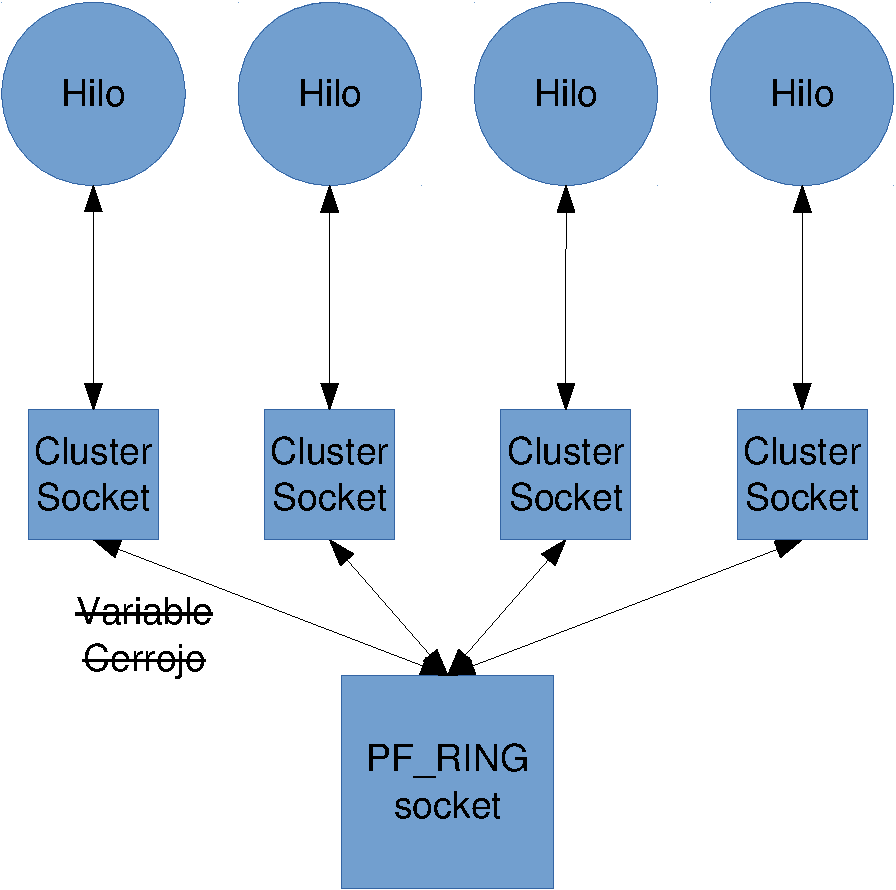
\includegraphics[width=\textwidth]{CapituloPF_RING/Figuras/CluserCluster-crop}%
 \LABFIG{PFRINGClusterCluster}
  \end{minipage}}
\caption{Ventajas de usar \texttt{PF\_RING} clustering}
\end{figure}
%

Un cluster \texttt{PF\_RING} persigue eliminar esa necesidad. En lugar de competir por los mismos recursos (el anillo 
\texttt{PF\_RING}), cada hilo tiene su propio socket, y el cluster se encarga de distribuir los paquetes a medida que 
éstos llegan. De esa forma, no es necesario bloquear los hilos cada vez que se desea leer un paquete, y todo el 
inter-bloqueo se realiza a nivel de núcleo, donde estas operaciones se hacen mucho más rápidas. Podemos ver una 
representación gráficas en las figuras \FIG{PFRINGClusterNoCluster} frente a \FIG{PFRINGClusterCluster} 
\cite{MonitoringUsingNtop}.

\subsection{Uso de PF\_RING}
Para usar \texttt{PF\_RING} en una máquina CentOS 6.5, fue necesario instalar:
\begin{enumerate}
 \item Compilador \texttt{gcc} y \texttt{gcc-c++} para compilar fuentes escritas en C++
 \item Cabeceras y fuentes del núcleo: \texttt{kernel-devel} y \texttt{kernel-headers}
 \item Librería NUMA para desarrolladores: \texttt{numa-devel}
\end{enumerate}

\begin{lstlisting}[language=bash,caption={Compilación e instalación de \texttt{PF\_RING}}, 
breaklines=true, label=code:CompilacionInstalacionPFRing,numbers=left,float=htbp]
# Compilamos el módulo del núcleo y lo instalamos
pushd kernel; make; ./insmod ./pf_ring.ko; popd


# Compilamos las librerías de espacio de usuario
pushd userspace; make; make install; popd

# Buscamos el driver ZeroCopy en drivers/XXXX, y lo instalamos
\end{lstlisting}

Tras ello, se podría ejecutar el comando \texttt{make} en su directorio base, pero es posible que fallen algunas 
compilaciones de los drivers, ya que CentOS realiza algunas modificaciones sobre el núcleo con el fin de hacerlo más 
estable. Por ello, lo recomendado es seguir los pasos de \lstlistingname{} \ref{code:CompilacionInstalacionPFRing}

Tras la instalación del módulo y las librerías, podemos comenzar a probar algunos de los ejemplos que vienen con la 
distribución, y comparar.

\subsection{Ejemplo de ZeroCopy}
Para probar la tecnología \texttt{PF\_RING ZeroCopy}, la distribución viene con algunos ejemplos\footnote{Se puede 
descargar de forma gratuita desde 
\url{https://svn.ntop.org/svn/ntop/trunk/PF_RING/userland/examples_zc/README.examples}} como un contador de paquetes 
que usa libpcap (\texttt{pcount}), que usa la interfaz \texttt{PF\_RING} (\texttt{pfcount}), que usa 
la interfaz ZeroCopy (\texttt{zcount}).

Probaremos la aplicación \texttt{pcount} en una interfaz a la que estamos enviando paquetes UDP de $64$ bytes a $1Gbps$ 
mediante \texttt{zsend}. Los equipos emisor y receptor serán dos equipos \texttt{Intel\textregistered{} 
Xeon\textregistered{} E31240} a $3,30GHz$, con $32G$ de memoria RAM\footnote{Se verán más detalles de los equipos en la 
sección \CHAP{EntornoPrueba}}.

Comenzando con la aplicación \texttt{pcount}, es capaz de procesar los paquetes a unos $713mbps$, usando para ello el 
$100\%$ de la CPU. El resto de paquetes,  aparecen en las estadísticas como descartados.

Sin embargo, con tan sólo usar \texttt{PF\_RING}, vemos que la aplicación es capaz de leer a $1Gbps$, pero usando 
aproximadamente el 50\% de la CPU.

Si ahora usamos la interfaz \texttt{ZeroCopy}, pero no usamos la interfaz en modo \texttt{ZeroCopy}, vemos que al 
aplicación es capaz de contar el 100\% de los paquetes, usando tan solo un 9\% de la CPU. Si, por último, usamos 
\texttt{ZeroCopy} puro, vemos que el uso de la CPU desciende hasta el 4\%.

Se resumen los resultados de las pruebas en la \TAB{ResultadosPFring}.

\begin{table}[htbp]
 \begin{tabular}{llll}
  Modo PF\_RING & Velocidad de recepción & Descartados  & Uso de CPU              \\\hline
  No                       & $\approx 713mbps$ & $\approx0.3\%$  & $\approx{}98\%$ \\
  PF\_RING                 & $1Gbps$           & $0\%$           & $\approx{}50\%$ \\
  PF\_RING ZC sobre núcleo & $1Gbps$           & $0\%$           & $\approx{}9\%$  \\
  PF\_RING ZC puro         & $1Gbps$           & $0\%$           & $\approx{}4\%$
\end{tabular}
  \caption{Resultados de las pruebas realizadas con \texttt{PF\_RING}}
  \LABTAB{ResultadosPFring}
\end{table}

\section{Aportaciones realizadas a PF\_RING}
\texttt{PF\_RING} es, en su mayor parte, código libre licenciado bajo GPL2. Por ello, su código se puede estudiar y 
modificar libremente. Durante el desarrollo del proyecto, se descubrió que \texttt{PF\_RING} no balanceaba bien los 
paquetes fragmentados, y se ayudó Alfredo Cardigliano, principal mantenedor del proyecto, a solucionar el fallo.

Por defecto, \texttt{PF\_RING} balancea haciendo un hash simétrico de dirección origen y destino, puerto origen y 
destino y protocolo. Sin embargo, la información del puerto no viaja en el paquete fragmentado, lo que los hacen 
difícil de manejar para el balanceador.

Para su correcto procesado, \texttt{PF\_RING} almacena el ID del fragmento y el socket al que lo ha dirigido. Sin 
embargo, este proceso no contemplaba más allá de dos fragmentos, y eliminaba esta información si llegaba el segundo 
fragmento.

\begin{itemize}
 \item El primer fragmento sería identificado como aquel que tuviese los campos de la cabecera IP 
\texttt{fragment\_offset}=0 y la bandera \texttt{more\_fragments}=1
 \item Por su parte, el segundo fragmento supondría \texttt{fragment\_offset}$ 
\neq$0, y \texttt{more\_fragments}=0.
\end{itemize}

Tras las modificaciones, \texttt{PF\_RING} identifica tres tipos de fragmentos:
\begin{enumerate}
 \item Primer fragmento, que cumple \texttt{fragment\_offset}=0 y \texttt{more\_fragments}=1.
 \item Fragmentos intermedios, que cumplen \texttt{fragment\_offset}$\neq$0 y \texttt{more\_fragments}=1.
 \item Último fragmento, que cumple \texttt{fragment\_offset}$\neq$0 y \texttt{more\_fragments}=0.
\end{enumerate}

Y sólo se elimina la información anteriormente descrita al llegar el último fragmento.

\begin{verbatim}
$ svn co https://svn.ntop.org/svn/ntop/trunk/PF_RING
$ cd PF_RING
$ svn log -r 8015
------------------------------------------------------------------------
r8015 | cardigliano | 2014-07-31 20:17:26 +0200 (jue 31 de jul de 2014) | 1 línea

fragment cache fix (courtesy of Eugenio Perez <eugenio@redborder.net>)
------------------------------------------------------------------------
\end{verbatim}


\section{Conclusiones}
El núcleo de un sistema operativo como Linux es el encargado de hablar con el hardware disponible y, por tanto, de 
recoger los paquetes. Sin embargo, el camino que los paquetes tienen que atravesar hasta llegar al espacio de usuario 
no está muy optimizado, y encontramos pérdidas de rendimiento en muchos puntos, fundamentalmente, excesivas copias de 
memoria y un uso abusivo de interrupciones del sistema, tanto para reservar memoria como para la notificación de 
paquetes disponibles.

\texttt{PF\_RING} intenta solucionar ambos problemas creando un camino directo entre la tarjeta y la aplicación en 
espacio de usuario. Reservando de antemano un anillo en el que almacenar los paquetes, ahorramos al núcleo la necesidad 
de buscar memoria libre para cada paquete recibido, y la sobrecarga que ello supone. A continuación, nos saltamos toda 
la pila de linux, que sabemos que no vamos a necesitar, ya que simplemente queremos el paquete íntegro en espacio de 
usuario. Por último, evitamos una copia al espacio de usuario permitiendo el mapeo del anillo a la memoria de usuario.

Sobre \texttt{PF\_RING} podemos aplicar una nueva mejora: \texttt{ZeroCopy}. Con ello, podemos conseguir la lectura 
directa del paquete desde la memoria de la tarjeta, evitando así la primera copia desde la tarjeta al núcleo. Por otro 
lado, este marco de trabajo permite crear un Cluster \texttt{PF\_RING}, que permite dividir el troncal de tráfico en 
$n$ flujos independientes y coherentes, y crear un socket distinto para cada uno, de forma que los hilos lectores no 
tienen que competir para obtener los paquetes.

Por último, gracias a que \texttt{PF\_RING} es en parte de código libre, se pudo realizar aportaciones al proyecto y, 
de esa forma, mejorarlo un poco.

\section{Resumen}
\begin{Resumen}[Resumen de PF RING]

\subsection*{Conceptos preliminares}
\begin{flalign*}
&\begin{cases}
	\text{Núcleo Linux}
	\begin{cases}
		\text{Interfaz entre el hardware y las aplicaciones} \\
		\text{Linux es un núcleo modular} \\
	\end{cases}\\
	\text{Interrupciones}
	\begin{cases}
	  \text{Interrumpe el funcionamiento normal del núcleo}\\
	  \text{para ejecutar una función predefinida}
	\end{cases}\\
	\text{Llamada al sistema}
	\begin{cases}
	  \text{Petición desde el espacio de usuario para realizar} \\
		\text{tareas que requieren privilegios de núcleo}
	\end{cases}\\
	\text{Programador de tareas}
	\begin{cases}
		\text{Marca en qué intervalo se ejecuta cada aplicación}
	\end{cases}\\
	\text{Mapeo de memoria}
	\begin{cases}
		\text{Permite acceder a un recurso como si fuese una región de la memoria}
	\end{cases}\\
	\text{Direct Memory Access}
	\begin{cases}
		\text{Permite a un dispositivo escribir y leer de memoria}\\
		\text{sin intervención de la CPU}
	\end{cases}
\end{cases}&
\end{flalign*}

\subsection*{Procesado de paquetes por Linux}
\begin{flalign*}
&\begin{cases}
	\text{Reserva de memoria (DMA) y escritura del paquete}\\
	\text{Notificación al núcleo}\\
	\qquad\text{Mediante una interrupción}\\
	\text{Introducción a la pila del núcleo}\\
	\qquad\text{Operaciones como \texttt{netfilter}}\\
	\text{Copia de paquete al espacio de usuario}
\end{cases}&
\end{flalign*}

\subsection*{PF\_RING}
\begin{flalign*}
&\begin{cases}
  \text{PF\_RING}
  \begin{cases}
		\text{Buffer circular $\rightarrow$ no reserva de memoria}\\
		\qquad\text{Si no cabe en anillo, se descarta}\\
		\text{Los paquetes no pasan por el núcleo}\\
		\text{Creación de hilos exclusivos para los paquetes}\\
	\end{cases}\\
	\text{ZeroCopy}
	\begin{cases}
	  \text{Eliminación de la copia NIC $\rightarrow$ núcleo}\\
	  \text{Clustering, reparto eficiente de paquetes}
	\end{cases}\\
	\text{Se observa mejora de rendimiento al progresar}
\end{cases}&
\end{flalign*}

\end{Resumen}

\endinput

